\chapter{Wnioski}
\begin{figure}[h!] 
\centering 
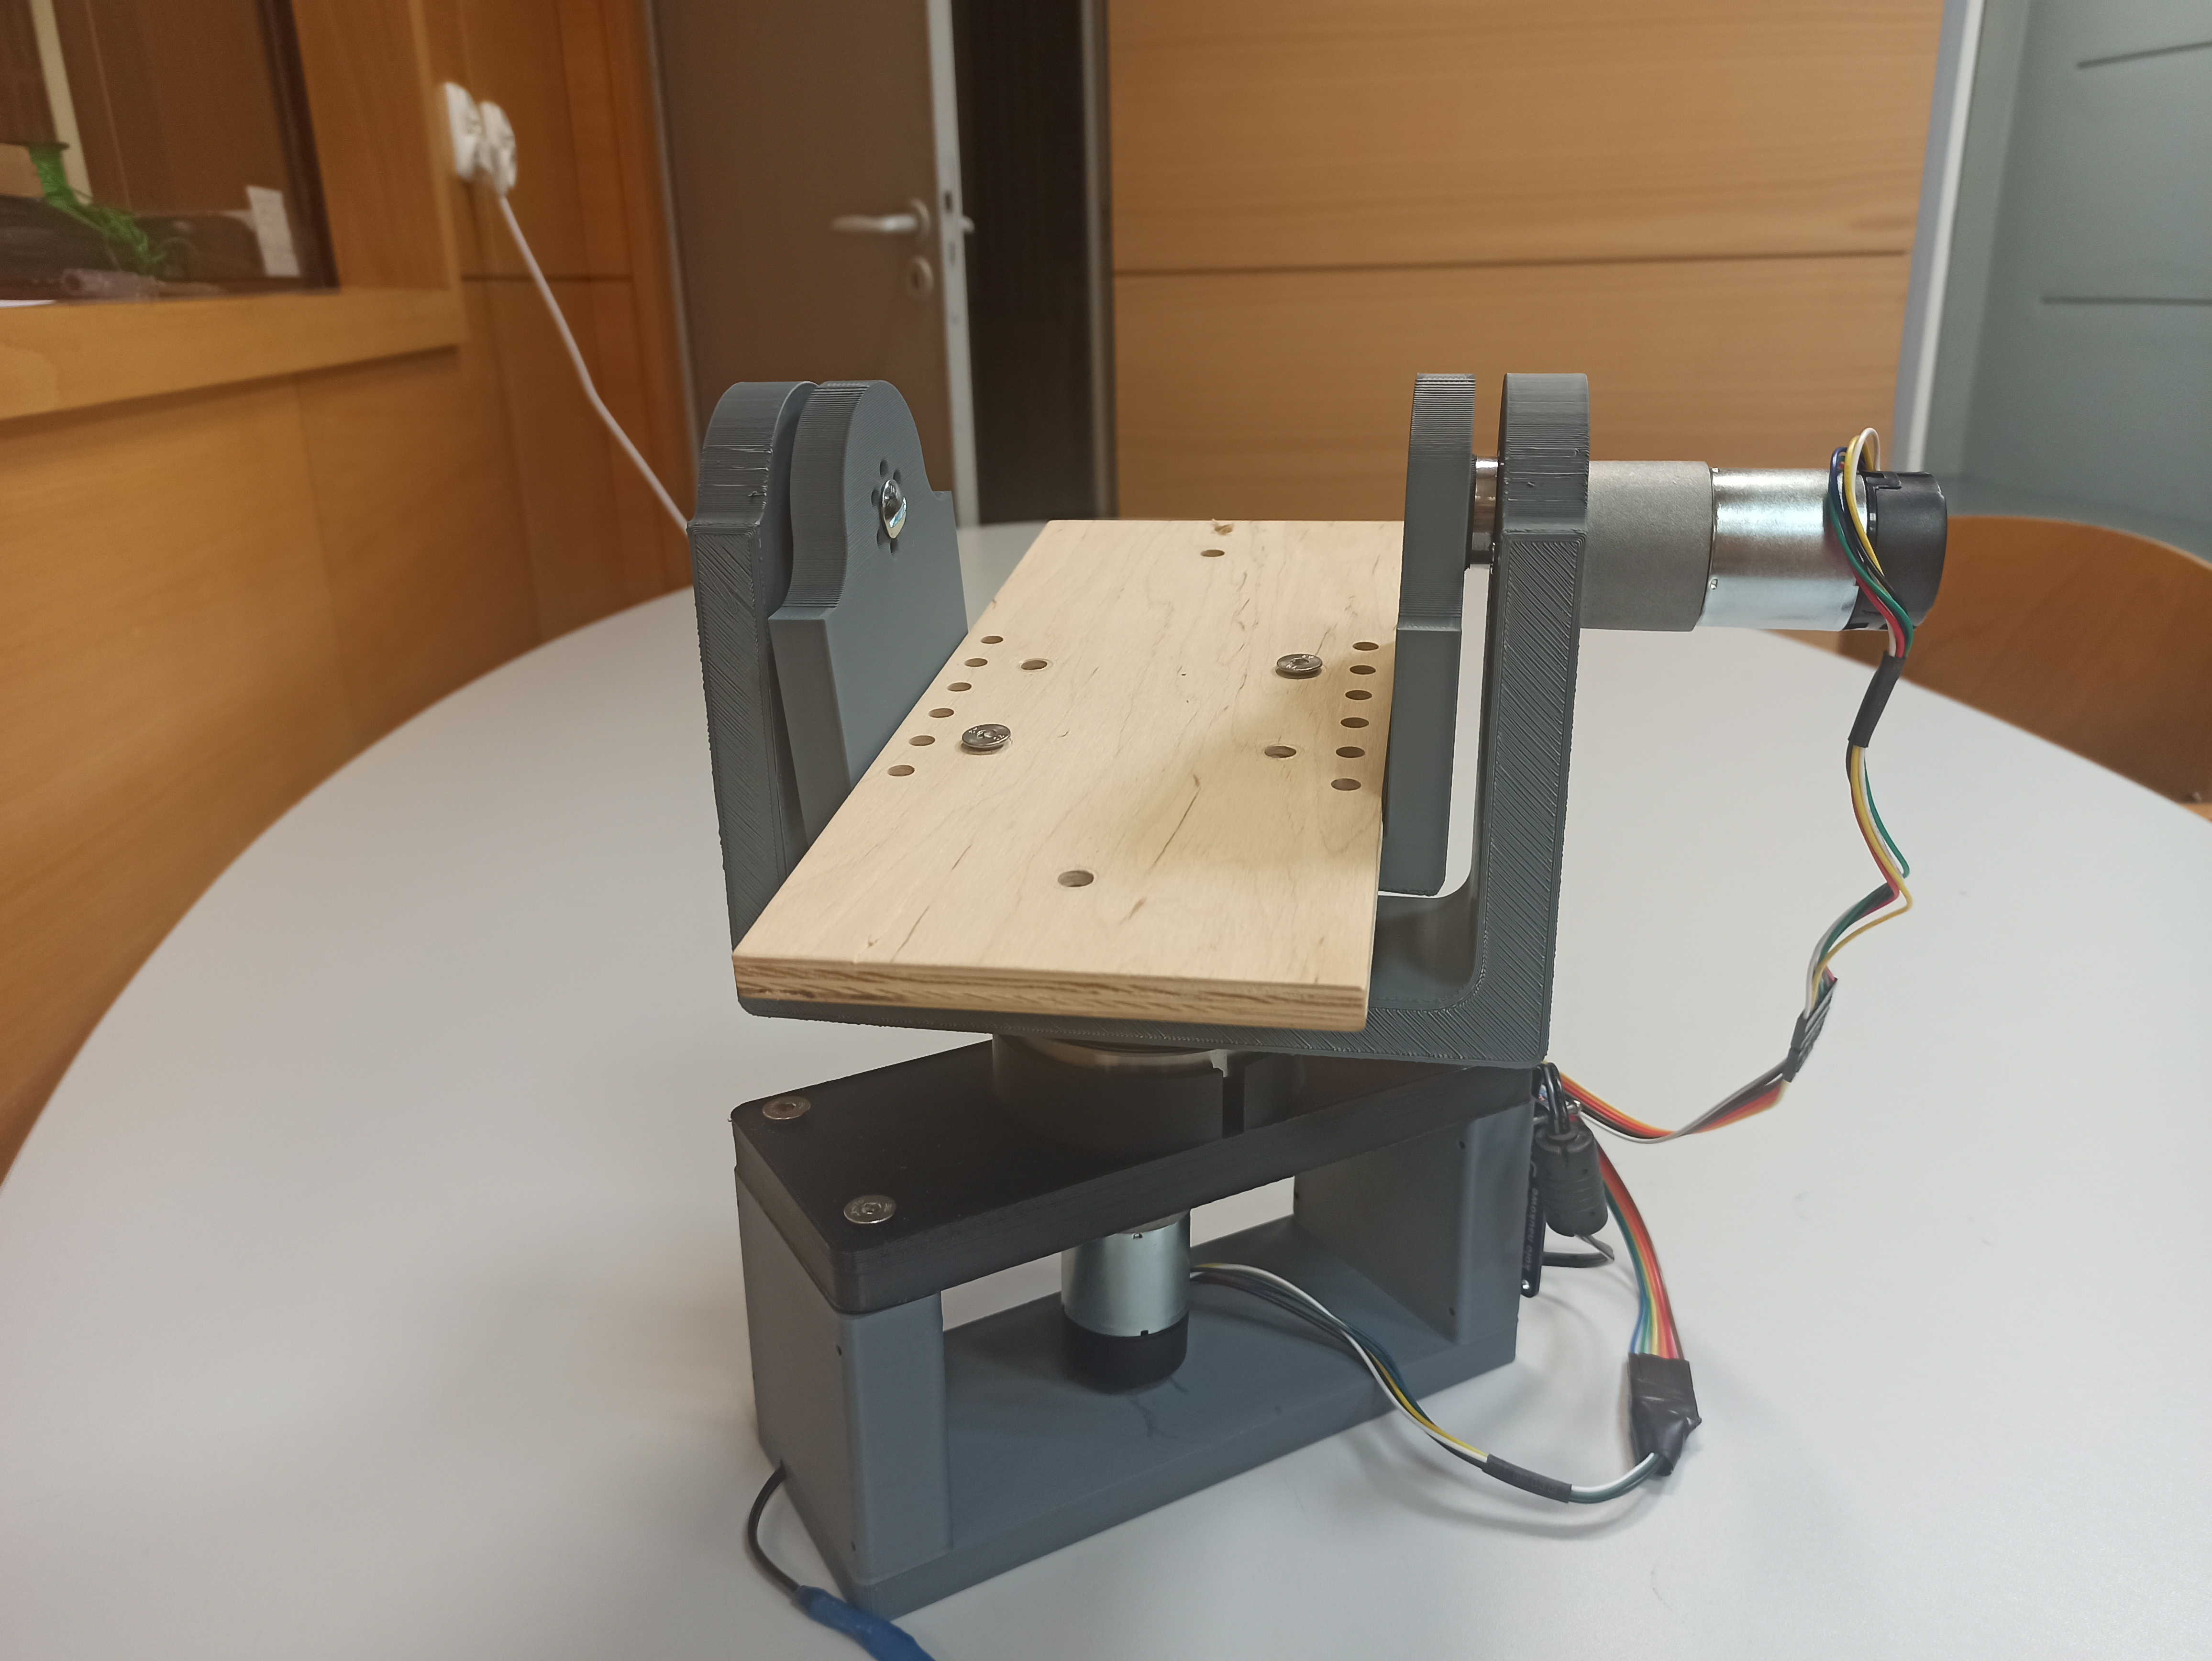
\includegraphics[width=\textwidth]{img/systemPhoto.jpg}
\caption{Skonstruowany system.}
\label{img:systemPhoto}
\end{figure}

Zaprezentowane w rozdziale \ref{cha:Measurments} pomiary, pokazują, że zbudowane urządzenie, przedstawione na zdjęciu \ref{img:systemPhoto}, działa poprawnie. Celem pracy było przeskanowanie powierzchni przy pomocy wibrometru punktowego  i cel ten został osiągnięty.

Oprogramowanie działa bez zarzutu oraz zgodnie z opisem przedstawionym w ramach tej pracy. Przy wielokrotnym uruchamianiu i podczas wykonywania wielu skanów nie wykazało żadnych błędów. Natomiast należy pamiętać, że zgodnie z teorią testowania oprogramowania, można jedynie wykazać istnienie błędów, nie można udowodnić ich braku. Dlatego też sugeruje się, aby podczas wykonywania pomiarów przymocowywać system do podłoża, tak jak zostało to zrobione podczas pomiarów opisywanych w rozdziale \ref{cha:Measurments}. Wibrometr, nawet punktowy, jest bardzo drogim urządzeniem, a przy gwałtownych ruchach spowodowanych błędami oprogramowania lub sprzętu, cała konstrukcja może się przewrócić. Zwłaszcza, że środek masy wibrometru znajduje się wyżej, niż zakładano podczas tworzenia pierwszych wersji modeli, co spowodowało, że podstawa całego systemu jest za mała. Podczas normalnej pracy rozmiar postawy jest w zupełności wystarczający, natomiast w razie pojawienia się większych momentów istnieje ryzyko przesunięcia środka masy poza obszar podstawy i przewrócenie się urządzenia.

W tym miejscu można także zastanowić się nad sensem użycia silników szczotkowy w tego typu projekcie. System zadziałał, więc wydaje się to zasadne. Natomiast nie było to łatwe zadanie, regulator opisywany w rozdziale \ref{cha:pos_control} ostatecznie zawierał więcej elementów i wykonywał więcej obliczeń, jak na przykład histereza czy tandem dwóch regulatorów. Kontrola pozycji okazała się także mniej precyzyjna niż pierwotnie zakładano. Pomimo dużej precyzji enkodera, i dość dokładnej (bo do około $\pm0.05^{\circ}$) znajomości pozycji, to wymuszanie takiej dokładności powodowało znaczne przeregulowania, spowodowane faktem, że silnik szczotkowy ma pewną minimalną prędkość i nie da się go zmusić do wolniejszego ruchu. Dlatego też nawet najlepiej dostrojone regulatory mogłyby mieć problem z przeregulowaniem. W celu poprawienia tej regulacji można by podjąć próbę zaimplementowania regulatora w samym przerwaniu od enkodera, zamiast przerwaniu od zegara. Sprawiłoby to, że informacja o sprzężeniu zwrotnym byłaby natychmiastowa. Jednakże istnieje ryzyko, że procesor nie dałby rady wykonywać tylu obliczeń w tak krótkich odstępach czasu. Można by także spróbować użyć trybu "Short Brake", udostępnianego przez użyty sterownik Toshiby. Jednakże tryb ten powoduje gwałtowne hamowanie, co znowu mogłoby spowodować inne problemy, jak na przykład pękające zębatki przekładni. Alternatywnym, najprostszym rozwiązaniem byłoby zastąpienie silnika szczotkowego silnikiem krokowym, w przypadku którego takie problemy nie występują.

Kolejnym problemem jaki wyniknął z użycia silników szczotkowych to luzy. Bardzo możliwe że są one wywołane przez przekładnię, a nie sam silnik, więc nie da się jednoznacznie określić czy zastosowanie silników krokowych rozwiązałoby problem.

Podczas wykonywania pomiarów pojawił się także problem trzęsących się modeli. Jest to przypadłość materiałów, z jakich modele te zostały wydrukowane, są one dość giętkie. Dlatego też istotnym krokiem w dalszym rozwoju tego projektu byłoby wycięcie całości konstrukcji z aluminium, zamiast druku.

Potencjalne miejsce, gdzie można by rozwinąć oprogramowanie, zostało opisane w rozdziale \ref{cha:auto_scanner}. Zaznaczono tam potencjał dołączenia układu ADC, który zbierałby pomiary, zamiast dodatkowej karty dźwiękowej podpinanej do komputera. Idąc krok dalej, można by także przeprowadzić całą analizę danych po stronie mikrokontrolera, jednakże to wymagałoby implementacji całej filtracji oktawowej w języku C. Wykonanie tego zadania umożliwiłoby przeprowadzanie całych pomiarów za pomocą zaledwie jednej komendy wysyłanej do urządzenia. Kolejny aspekt potencjalnej rozbudowy, to komunikacja między wibrometrem a systemem pozycjonowania. Wibrometr posiada gniazdo RS-232. Zapoznanie się z komendami, pozwoliłoby na kontrolę wibrometru z poziomu powstałego systemu.
